Liu et al. \cite{liuRethinking3DCNNHyperspectral2023} propose the Full 3D U-Net (F3DUN),
for hyperspectral image super resolution.
The model implements a U-Net architecture composed solely of three-dimensional convolutional layers.
Because of the multi-band property of hyperspectral images,
3d convolutions come as a natural candidate for processing this type of data.
On the other side, previously pure 3d CNN models were considered difficult to train. 
As the combination of increased model capacity, compared to 2d convolutional networks,
and the the absence of large datasets for HSI related tasks,
the risk of overfitting is present.
Liu et al. \cite{liuRethinking3DCNNHyperspectral2023} disprove this common assumption in their work,
by introducing a more carefully designed model architecture,
outperforming previous state-of-the-art methods.
The overall architecture is displayed in figure \ref{fig:f3dun}.

\begin{figure}[h!]
    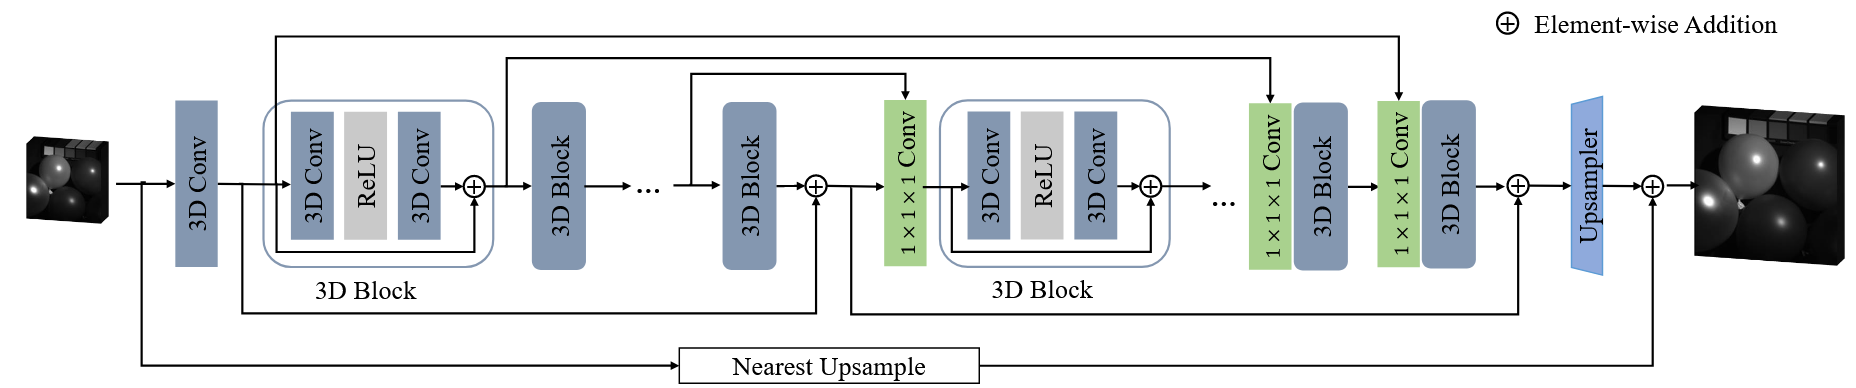
\includegraphics[width=0.9\textwidth]{models/hsisr/imgs/f3dun.png}
    \caption{Image taken from \cite{liuRethinking3DCNNHyperspectral2023}, architecture of F3DUN.}
    \label{fig:f3dun}
\end{figure}

For shallow feature extraction one 3d convolutional layer $H_S = C_3(31, 64, \text{kernel-size}=3, \text{padding}=1)$ is used.
The features are scaled to the desired spatial dimension using a transposed 3d convolution.

\noindent Throughout the architecture the following convolution is mostly used

 \begin{equation*}
    C = C_3(64, 64, \text{kernel-size}=3, \text{padding}=1) ~.
 \end{equation*}

The basic building block of the model is the 3d Block,
$10$ of such block are employed 

\begin{equation} \label{eq:3dblock}
    H_{3dBlock, i} = R(C \circ \text{ReLU} \circ C) ~,
\end{equation}

\noindent for $i = 1, ..., 10$. 
Given an input $X \in \mathbb R^{31 \times H \times W}$, 
the shallow features $F_0 \in \mathbb R^{64 \times H \times W}$ are computed by

    $$ F_0 = H_S(X) ~. $$

The features are then passed through the contracting path of the U-Net

    $$F_{i} = H_{3dBlock, i}(F_{i-1}) ~,$$

for $i = 1, ..., 4$. In contrary to the standard U-Net architecture,
the authors introduce two more skip connections, 
reaching from the beginning of each path to its end.
For the contracting path this is

    \begin{equation} \label{eq:skip_contracting}
        F_{5} = H_{3dBlock, 5}(F_4) + F_0 ~.
    \end{equation}

Next the features are further processed by the expanding path.
As it is common in U-Nets, 
the features from the previous block are concatenated with the features put out by the block at the same level in the contracting path.
To this end, the following module is used

\begin{equation} \label{eq:fuse}
    H_{fuse, i} = C_3(128, 64, \text{kernel-size}=1) ~,
\end{equation}

for $i=6, ..., 10$.
To map the concatenated features down from $128$ to $64$ channels, 
the fuse module defined in (\ref{eq:fuse}) is employed before the 3d block

    $$F_{i} = H_{3dBlock, i} \circ H_{fuse, i} \left( \big[F_{10 - i}, F_{i-1} \big] \right) ~.$$

For $i = 6, ..., 9$, note $F_{10 - i}$ is the feature, coming from the same level of the contracting path.
Analogously to the contracting path, as in equation (\ref{eq:skip_contracting}),
a skip connection is also used in the expanding path

    $$ F_{10} = H_{3dBlock, 10} \circ H_{fuse, 10} \left( \big[F_{9}, F_0 \big] \right) + F_5 ~. $$

The features $F_{10}$ are the final output of the deep feature extraction module.